\documentclass[a4paper]{article}
\usepackage[margin=2cm]{geometry}
\usepackage{tikz}
\usetikzlibrary{shapes.geometric, arrows.meta}

% Gaya node
\tikzstyle{startstop} = [rectangle, rounded corners, minimum width=4cm, minimum height=1cm, text centered, draw=black, fill=blue!20]
\tikzstyle{process} = [rectangle, minimum width=4cm, minimum height=1cm, text centered, draw=black, fill=orange!20]
\tikzstyle{arrow} = [thick,->,>=stealth]

\begin{document}
	
	\begin{center}
		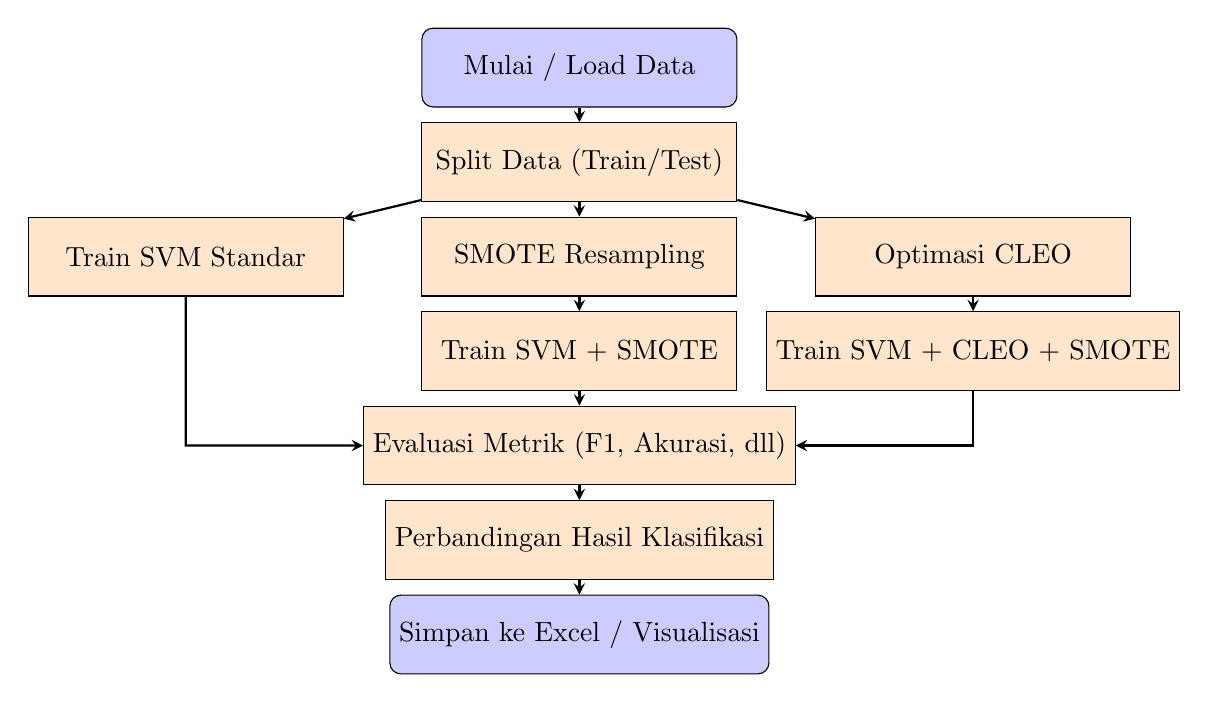
\begin{tikzpicture}
			
			% Baris 1
			\node (start) [startstop] at (0,0) {Mulai / Load Data};
			
			% Baris 2
			\node (split) [process] at (0,-1.2) {Split Data (Train/Test)};
			
			% Baris 3
			\node (svm) [process] at (-5,-2.4) {Train SVM Standar};
			\node (smote) [process] at (0,-2.4) {SMOTE Resampling};
			\node (cleo) [process] at (5,-2.4) {Optimasi CLEO};
			
			% Baris 4
			\node (svm_smote) [process] at (0,-3.6) {Train SVM + SMOTE};
			\node (svm_cleo_smote) [process] at (5,-3.6) {Train SVM + CLEO + SMOTE};
			
			% Baris 5
			\node (eval) [process] at (0,-4.8) {Evaluasi Metrik (F1, Akurasi, dll)};
			
			% Baris 6
			\node (compare) [process] at (0,-6.0) {Perbandingan Hasil Klasifikasi};
			
			% Baris 7
			\node (save) [startstop] at (0,-7.2) {Simpan ke Excel / Visualisasi};
			
			% Panah vertikal (1cm antar baris)
			\draw [arrow] (start) -- (split);
			\draw [arrow] (split) -- (smote);
			\draw [arrow] (smote) -- (svm_smote);
			\draw [arrow] (svm_smote) -- (eval);
			\draw [arrow] (eval) -- (compare);
			\draw [arrow] (compare) -- (save);
			
			% Panah horizontal dan diagonal pendek
			\draw [arrow] (split) -- (svm);
			\draw [arrow] (split) -- (cleo);
			\draw [arrow] (cleo) -- (svm_cleo_smote);
			\draw [arrow] (svm) -- ++(0,-2.4) -- (eval); % SVM → Evaluasi
			\draw [arrow] (svm_cleo_smote) -- ++(0,-1.2) -- (eval); % CLEO → Evaluasi
			
		\end{tikzpicture}
	\end{center}
	
\end{document}